\section{研究问题与实验分层}
实验以竞赛作品展示为主，重点回答：固定软件工件上的识别结果能否复现，
证据是否可追溯，以及发布前体检和整改对比是否形成可操作的演示闭环。
另保留完整开发与历史不同作者结果，供解释识别范围和后续改进使用。

\begin{table}[htbp]\centering\small
\caption{实验层次、输入和结论边界}\label{tab:experiment-layers}
\begin{tabularx}{\linewidth}{p{2.2cm}p{3.4cm}X}\toprule
层次 & 输入与固定条件 & 要回答的问题\\\midrule
十三算法复扫 & 开发总体的全部源码及双架构程序，共 1071 份 & 第四章主实验：十三算法的范围内漏报及分载体差异。\\
混合演示复扫 & 五算法、两架构、241 份源码/程序；来源分列 & 保留旧紧凑演示的可复现结果，不代替十三算法主实验。\\
网关应用验收 & 两版源码、四份 SDK、四个视图 & 证据、迁移待办、差异、离线网页和现场调用是否连通。\\
开发回归 & 2344 文件、六份开发清单，按内容去重 & 附录保留已知家族覆盖和原有规则回归结果。\\
历史验证复查 & 2855 / 232 / 252 文件，沿用原锁及源码边界 & 附录保留既有不同实现覆盖；不是新的盲测。\\\bottomrule
\end{tabularx}\end{table}

历史结果来自已经完成并留存的实验，本轮重新核算其 JSON；
已完成的 241 份混合演示及五类固件实验继续保留；
本轮另对按载体和架构全取的 1071 份开发输入实际新扫。
没有重新训练模型、修改识别器或重跑完整历史样本库。
图表生成脚本从同一份证据摘要生成表格，原报告路径与哈希保存在附录及
\nolinkurl{data/evidence.json} 中。

\section{系统架构与工程环境}
\subsection{检测引擎与应用层分工}
主工程位于 \nolinkurl{ustc_tool_middle/}，Python 包位于 \nolinkurl{src/qcs/}。
统一入口提供 \texttt{doctor}、\texttt{scan}、\texttt{evaluate}；
固定多清单实验另有开发与历史复查运行器。
GridLens 位于 \nolinkurl{examples/gridlens/}，只消费真实报告和显式场景标注，
不为展示重新创造一套算法识别规则。

\begin{table}[htbp]\centering\small
\caption{实现模块与可审查职责}\label{tab:module-layout}
\begin{tabularx}{\linewidth}{p{5.2cm}X}\toprule
模块 & 主要职责\\\midrule
\nolinkurl{scanner.py}, \nolinkurl{model.py} & 对象分派、预算、状态、证据与双口径预测。\\
\nolinkurl{source.py}, \nolinkurl{api_rules.py}, \nolinkurl{source_reference.py} & 词法角色、参数映射、已审核源码引用及身份核验。\\
\nolinkurl{symbols.py}, \nolinkurl{yara_engine.py}, \nolinkurl{function_signatures.py} & 符号、规则、可执行段内完整函数及常量核验。\\
\nolinkurl{operations.py}, \nolinkurl{guomi/}, \nolinkurl{semantic_probes.py} & 源码/二进制运算见证、国密和隔离指令探针。\\
\nolinkurl{miasm_backend.py}, \nolinkurl{miasm_worker.py}, \nolinkurl{miasm_summary.py}, \nolinkurl{miasm_scan.py} & 外部环境控制、有限 CFG、位向量摘要和现有算法桥接。\\
\nolinkurl{firmware.py}, \nolinkurl{firmware_native.py} & 固件结构校验、受限提取、组件递归和来源链。\\
GridLens 的 \nolinkurl{assessment.py}, \nolinkurl{server.py}, \nolinkurl{app.js} & 资产组织、规则待办、本机扫描服务与离线网页。\\\bottomrule
\end{tabularx}\end{table}

\subsection{解释器、依赖与资源控制}
主引擎使用 Python 3.12.3 隔离环境。已保存 doctor 记录确认
YARA 4.5.4、pyelftools 0.32、pefile 2024.8.26、Capstone 5.0.6、
Tree-sitter 0.25.2、Unicorn 2.1.4 等运行依赖可用。
国密解析器与规则、源码参考库、函数库均带摘要；普通函数签名库为 1028 条，
国密参考与开发签名库分别为 152 和 211 条。
这些是数据库记录数，不是算法种类数、独立实现数或正确检出数。
Miasm 固定提交为 \nolinkurl{3671fc24d6e625c2d75f3311724eb6b0c97664f8}，
运行在独立环境，保留 GPL-2.0-only 许可\cite{miasm}。
Binwalk 在该份最终 doctor 中缺失或不支持，但原生适配器和 SquashFS 工具可用。

本机修订时可见环境为 Fedora CoreOS 42、x86-64、Intel Xeon Silver 4410Y，
可见逻辑 CPU 为 48 个；这份机器信息是本轮采集，未冒充历史每次运行的资源监测。
历史批次并发条件按原记录保留：三批历史复查使用 32 进程，
旧筛选演示复扫两批各 16 进程并行；本轮混合演示使用 16 进程单批复扫。

默认每对象预算为 60 秒、10000 文件、4 层固件递归、1 GiB 总字节和 256 MiB 单文件。
目录与镜像组件共享预算；固定集合评测则逐文件独立预算。
Miasm 阶段最多两个候选、合计 3 秒、单次不超过 1.5 秒，消耗原总时限的剩余部分。
GridLens 的单文件外部进程上限为 85 秒，演示配置关闭 Miasm，
因此其六文件速度不能与默认开启后端的全量实验直接比较。

\section{样本、真值与冻结方案}
\subsection{真值单位和标注范围}
主实验的单位是\textbf{文件--算法标签}。
每行含输入路径、内容 SHA-256、项目、实现家族、架构、编译参数、符号状态、
真实存在集合 $T_i$ 及已标注算法范围 $K_i$。
未在 $K_i$ 中的算法不当作阴性；同一文件可以同时存在多个正标签。
源码、构建模块及编译宏共同决定实现真值，函数名本身不作为独立语义正确性证明。

原始资料库包含 12870 份不同内容、12900 个物理文件，
其中有头文件、建库参考、许可配套和排除来源。
这些存量数不进入实验分母。
开发清单按内容合并时核对共同标注范围，避免把同字节的不同构建名称重复计数。
相同作者的多个优化级别仍属于同一实现家族，不作为独立作者样本。

\subsection{源码上下文与程序构建边界}
源码运算识别可能使用局部头文件和明确调用关系，
所以比较前固定源文件以及允许的上下文路径。
历史复查沿用原隔离源码边界；若当前工作树旁出现开发文件，不能扩大为可见上下文。
缺少局部依赖的源码片段，其实现级漏报与 API 调用级检出并非同一问题。
程序构建保存优化参数与架构，对剥离符号、共享库或仅模块构建分别注明；
未编译成功的尝试不伪装成完成的扫描输入。

\subsection{冻结及本轮证据核验}
历史复查使用的最终检测包摘要为
\nolinkurl{16dc3c38dd4f8d1e9ef4da1ff3307a8b438ae34381361386992e93f2c09af2c3}。
记录冻结了代码、样本与外部环境，并在运行后再次核验。
开发汇总在修正 MIPS 输出寄存器接口后重扫了受影响的 560 个文件，
另 1784 份结果按未受影响的代码行为复用并保留原始报告哈希；
不能称最终版本再次完整新扫了全部 2344 文件。
三批历史复查则全部新扫，未根据本轮历史预测继续调规则。
这些集合已经在之前开发周期中被观察，因此本文称其为历史验证复查。

\section{三类载体的实验实施方案}
\subsection{源码实验}
先计算摘要并解码，分别构造代码与参数视图，
识别专用接口、直接算法选择参数、调用/定义/声明角色；
在可用范围内进一步检查语法树运算、查表来源、指针关联及有限内部调用。
设置注释、声明、普通字符串、动态变量、共享常量和通用大数阴性对照。
验收既检查能否找到阳性，也检查不充分线索是否保持未知。

\subsection{ELF/PE 程序实验}
校验格式与架构后，依次运行符号、字节、函数签名、国密运算、
静态语义及隔离探针，再在剩余预算中尝试 Miasm。
参考函数须在可执行段匹配，重定位字段需掩盖，使用只读常量核对区分共享轮函数。
PE 的已验证路径主要依赖结构化导入与相应字节规则，
不把 ELF 整函数签名或各 ISA 的部分语义能力转述为 PE 全面覆盖。
遇到通道失败保留其他结果，并记录部分完成。

\subsection{固件实验}
对受支持的 SquashFS、gzip 和 ESP 容器先检查长度、头部、校验及段范围，
按限制提取组件并记录镜像摘要、相对路径、偏移和提取链。
可识别组件进入同一引擎；未支持的区域保持说明，不返回完整阴性结论。
当前三批主结果以源码和可执行文件为主，未单列真实终端固件总体准确率；
固件结论由工程适配与相应回归记录支持，不能拿主表替代固件效果统计。

\section{评测指标与错误处理}
设第 $i$ 个文件在口径 $s$ 上的预测为 $P_i^{(s)}$，
只在 $K_i$ 范围内比较。接口引用与实现包含分别计算，不相互充当命中。
主结果采用实现包含口径，计数为
\begin{align}
TP&=\sum_i |P_i\cap T_i\cap K_i|,&
FN&=\sum_i |T_i\setminus P_i|,\\
FP&=\sum_i |(P_i\setminus T_i)\cap K_i|,&
TN&=\sum_i |K_i\setminus(T_i\cup P_i)|.
\end{align}
由此定义
\begin{align}
\operatorname{Recall}&=\frac{TP}{TP+FN},&
\operatorname{FNR}&=\frac{FN}{TP+FN},\\
\operatorname{Precision}&=\frac{TP}{TP+FP},&
\operatorname{Accuracy}&=\frac{TP+TN}{TP+FP+FN+TN}.
\end{align}
误报率为 $FP/(FP+TN)$，与 $1-\operatorname{Precision}$ 不同。
分母为零时标为不适用。总体准确率可能被大量阴性标签抬高，
故必须同时报告召回率、漏报和绝对计数。
同一文件的多个变体相关，不给出假设标签独立的置信区间来夸大样本量。

扫描完成度也不等于正确率。
\texttt{partial}、失败和预算耗尽不从固定分母删除，已取得预测仍保留；
否则会把难样本通过运行状态过滤掉。
报告按算法、载体和架构分组，定位错误而不修改已锁定真值。

\section{语义后端对照方案}
Miasm 首先接受 ISA 夹具与数值真值测试，再进行开发对照，最后冻结后做三批历史复查。
对照核对逐文件预测、候选状态、原语数及阶段耗时。
接入前后扫描器并非只改变一个开关的严格单因素消融，旧探针存在时间波动，
因此明确区分后端直接产生的标签与其他引擎新增标签。
若后端仅返回大数原语，不能计作 RSA、ECDH、ECDSA 或 SM2 检出。
本轮没有完成每个通道逐一关闭的全量消融，也没有其他工具同条件排名实验。

\section{十三算法与分载体复扫方案}
\label{sec:algorithm-suite-method}
\subsection{算法范围与业务解释}
本轮算法范围与第二章逐项对应：分组密码 AES、DES、SM4；
流密码 RC4、ChaCha20；公钥机制 RSA、ECDSA、ECDH、SM2；
摘要 MD5、SHA-1、SHA-256、SM3。
DES、RC4、MD5、SHA-1 用作遗留资产识别对象；
RSA 及曲线机制支持解释身份认证、升级签名和密钥协商的量子迁移关注，
不要求五类最小业务样例各自包含所有算法。
Shor、Grover 是风险解释的理论依据，当前工具没有执行量子算法，
不将其列入静态密码实现识别的十三种标签。

\subsection{输入全取、冻结与目标}
在已保存的 2344 份开发输入中，纳入所有源码，以及所有 x86-64、ARM64 程序。
这一架构范围沿用原展示定位；不再按算法命中、项目、优化等级、符号状态或阴性配额筛选。
1071 份不同内容输入包括 154 份源码、527 份 x86-64 程序和 390 份 ARM64 程序；
其余 1273 份为其他机器架构，仍保留在完整开发报告中。
原开发结果已经被观察过，因此这是已知家族回归；全取政策不使它成为独立验证。

原样保留每个输入的 \texttt{truth} 和 \texttt{known\_algorithms}；
范围外或未完整标注的算法不改标为阴性。
源码复制完整的配套上下文，所有扫描入口与上下文文件在复扫前锁定，
同时锁定总体清单、纳入清单、检测器与运行时。
使用默认 Miasm 开启配置、逐文件 60 秒预算与 16 个进程，
全部新扫报告逐文件保存；部分、失败和漏报均留在固定分母中。
扫描前后的哈希必须一致，不根据新结果重选样本。

每算法的验收目标为 \(\operatorname{FNR}_a\leq10\%\)，
由 \(FN_a/(TP_a+FN_a)\) 计算，并显示正标签数、TP/FP/FN 和目标状态。
10.00\% 属于等于上限，不能写成严格低于 10\%。
精确率 \(TP/(TP+FP)\) 描述误报，不用于替代漏报目标，
保留实测值，不为获得特定外观添加错误标签。
另将源码、x86-64、ARM64 的漏报分列；混合范围达标不推出单一载体均达标。

\section{筛选演示集与网关场景方案}
\subsection{五算法混合演示清单}
五算法演示范围限定为 AES、SM4、SM3、MD5、SHA-1，以及 x86-64 / ARM64 ELF64。
二进制从旧五算法精简集取样；旧集已按项目、家族、架构和原真值分组，
每组选择已观察表现较好的编译变体，因此带有表现选择偏差。
本轮保留其中全部阳性输入，包括已有漏报；阴性按来源和架构各取 SHA-256 排序前 10 份。
开发源码每算法选择 5 份已观察成功样例，优先不同真实上游项目，
不足部分再按项目、家族和 SHA-256 排序补齐，另加 5 份范围内阴性。
同项目多个文件不称为不同作者，源码上下文也不当作新增扫描根。

清单共 241 份，开发二进制、历史二进制和开发源码分为三个来源字段，
文件内容按 SHA-256 去重。既有完整真值和标注范围继续保留，
本轮计数只在原范围与五算法范围的交集中进行；其他算法不改标为不存在。
原始样本库和验证集均保留，本轮只建立单独的演示输入副本。
所有输入、源码上下文、清单和检测器在扫描前锁定，复扫后不根据新成绩再次挑选。
这是一项混合演示实验，不具备独立验证所要求的开发/测试隔离。

\subsection{虚拟网关双版本}
四模块固定为遥测通信、升级校验、身份认证、第三方插件。
两个版本各有三份 C 适配源码，另有一份共享动态提供者源码和两架构各两份共享 ELF，
合计 11 个路径输入；身份源码在两版相同，不称为 11 个独立算法实现。
每视图使用 4 份源码与目标架构的 2 份 ELF。
源码适配代码未编译运行；SDK 由已有开发样本复制并核验哈希，业务归属为人工场景标注。

v1 使用 MD5/SHA-1 升级摘要和 AES-128-CBC 遥测适配；
v2 改为 SHA-256/SM3 和 AES-256-GCM。
两版仍保留 ECDH、RSA、ECDSA 接口，以说明摘要治理和公钥量子迁移是不同任务。
动态提供者使用运行时名称，不预设具体算法。

% 配图 P02：双版本真实源码片段的左右对照，不使用抽象迁移流程代替实际代码。
\begin{figure}[htbp]\centering
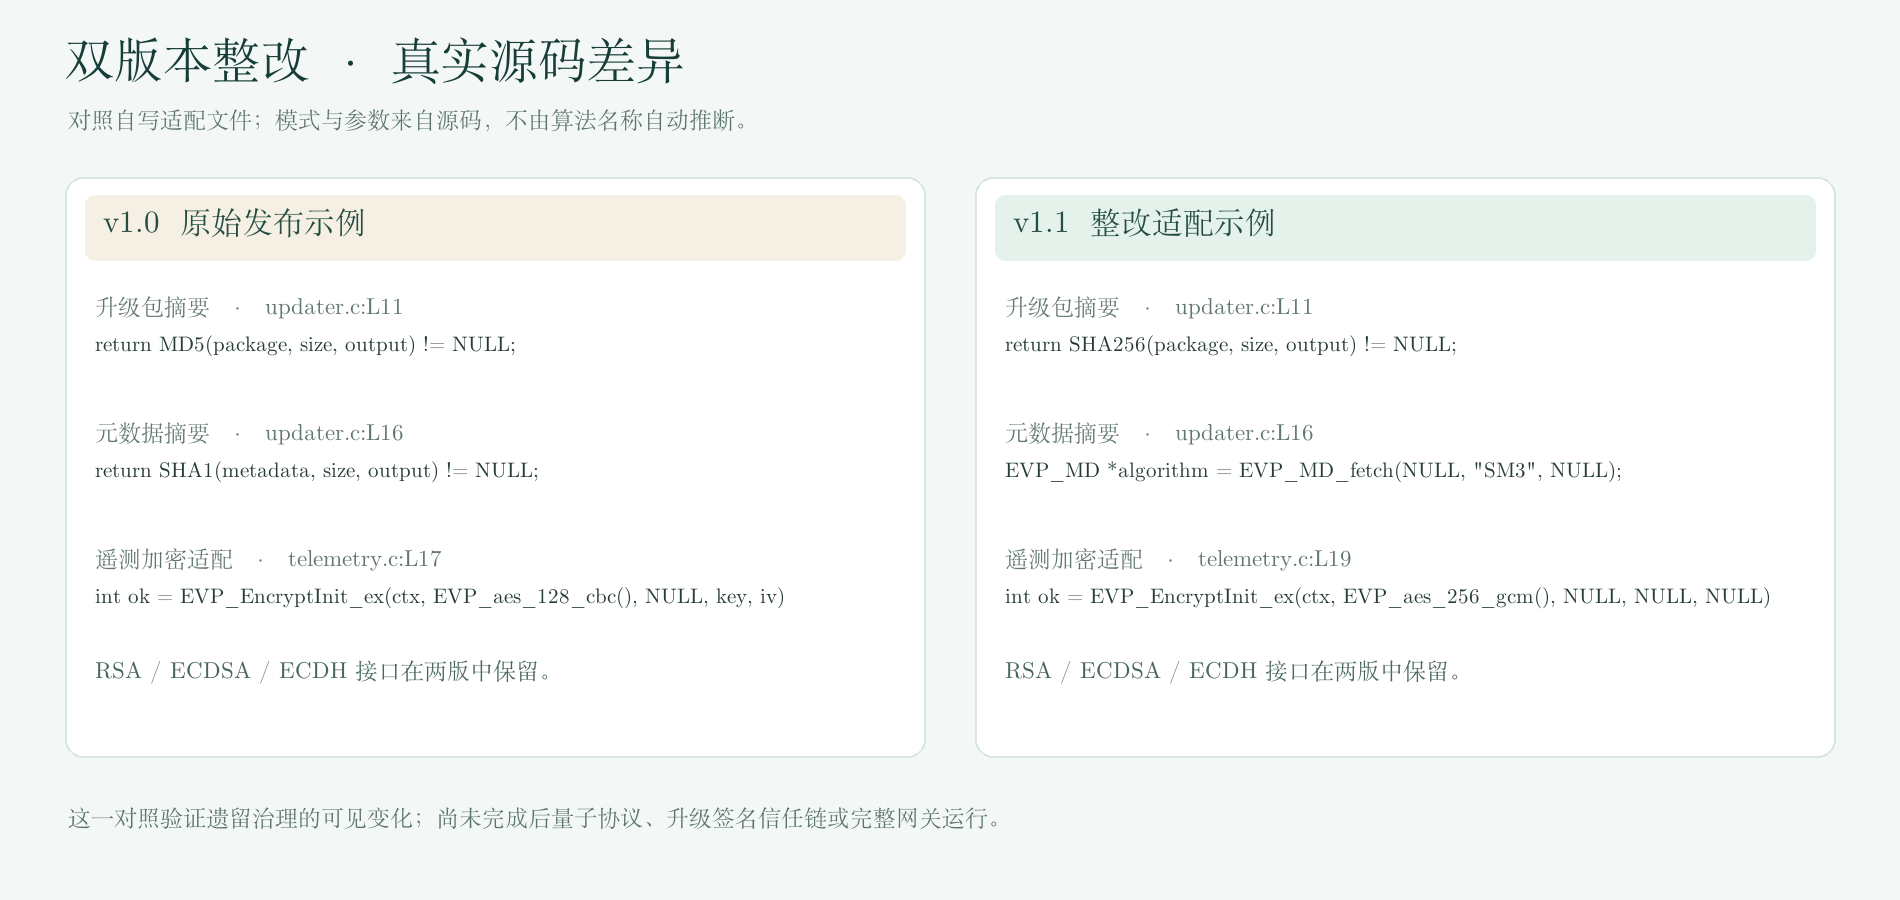
\includegraphics[width=\linewidth]{02-release-diff.png}
\caption{原始发布与整改适配的源码片段对照。两版公钥接口仍保留，摘要更换不等于完成后量子迁移。}
\label{fig:release-diff}
\end{figure}
% 配图注释（P02）：放左右两列代码样张，分别显示 MD5/SHA-1 与 SHA-256/SM3、
% AES-CBC 与 AES-GCM 的实际接口行；保留行号和文件名，并注明这是自写适配代码。

\subsection{交互与现场验收}
网页无外部 CDN，已有扫描数据作为本地脚本加载，适配 Windows 直接文件打开。
Linux 标准库服务只接受场景中的固定版本和架构，一次运行一个任务，
逐文件调用 QCS 并保存原始 JSON；失败不覆盖已有有效报告。
验收覆盖五页导航、四种视口、证据筛选与高亮、人工状态、导入导出、导览、回放与 PDF。
真实现场任务与离线回放分开标记，人工“已纳入计划”不修改扫描结论。

\section{五类电力终端的固件软件验证方案}
\label{sec:terminal-plan}
为检验从固件交付到密码证据的实际路径，另建五类终端软件场景：
智能电能表、用电信息采集集中器、配电自动化终端 FTU、继电保护装置 IED 和电力边缘网关。
业务程序分别执行电量累加、多表汇聚、事件序号检查、过流记录和主题路由，
不是把同一程序改五个名称。
每类具有独立源码、固定输入、预期业务输出和清单，在扫描前锁定。
密码源码来自已归属的教学实现与 OpenSSL，不把复用源码计为独立算法家族。

每类以 Zig 0.13.0 编译 x86-64 和 ARM64 的 Linux ELF 业务程序及共享库，
去掉静态符号，放入最小文件系统，再用 mksquashfs 生成 gzip 压缩的 SquashFS 镜像。
镜像与交付说明组成 ZIP，形成 10 份不同内容的交付包。
源码独立保留在构建目录，固件内只放程序、库、配置、固定业务数据及许可说明。
镜像没有内核、引导程序和完整系统运行库，不作为可启动设备固件。

验证先读取交付清单并核对 ZIP 与镜像 SHA-256，识别 SquashFS 后使用 unsquashfs 实际解包，
逐文件核对路径和内容哈希；再将镜像交给现有 QCS 固件入口，
由它再次解包并递归分析 ELF 与文本，保留固件哈希、组件路径、文件哈希及证据。
内容哈希校验不等于厂商签名认证，本实验没有提供真实厂商证书。
不要求从二进制恢复源码：固件通常只含机器码、库和配置，直接进行二进制静态识别即可。

每镜像包含两个已声明 ELF。五算法范围 AES、SM4、SHA-256、SHA-1、MD5 的实现标签
由构建源码和链接清单确定；文本及许可文件只计入提取清单，不作为实现阴性标签。
使用每镜像 180 秒预算、3 个并行任务，Miasm 关闭，
扫描前后核对识别器、runtime 和清单摘要，没有据新结果重新选择输入。
另运行五类提取后的 x86-64 程序，检查业务断言和所用密码的已知答案；
ARM64 仅交叉编译与静态扫描，未声明其运行验证。
这一软件级流程实验独立于 241 份混合演示清单，指标不合并。

\section{复现操作与记录保存}
单对象入口如下，输出统一放入新的目录，避免覆盖历史记录。
\begin{lstlisting}[basicstyle=\ttfamily\footnotesize,breaklines=true,breakatwhitespace=false,caption={环境检查与单对象复现入口}]
cd /var/home/gzn/ourtask
./qcs doctor --output ustc_tool_middle/build/reports/paper-check/doctor.json
./qcs scan examples/gridlens/releases/v1/updater.c \
  --output ustc_tool_middle/build/reports/paper-check/updater.json
./qcs scan examples/gridlens/components/sdk/x86_64/libmeter_adapter.so \
  --no-miasm --output ustc_tool_middle/build/reports/paper-check/sm4.json
cd examples/gridlens
python3 server.py --port 8765
\end{lstlisting}
这些命令是复现说明，不表示本次修订又执行了一轮完整评测。
主集合需使用保存逐行 $K_i$ 的原实验运行器，
不能把选择清单直接交给不认识其字段的通用评测入口。
附录给出运行器、清单、原始报告和图表脚本的对应关系。
